\documentclass{thomasClass}
\usepackage[utf8]{inputenc}

\title{\textbf{Required Practical 3}
\\Production of a dilution series of a solute to produce a calibration curve with which to identify the water potential of plant tissue
}
\author{Thomas Boxall}
\date{February 2021}
\begin{document}

\maketitle

\section{Method}
\begin{enumerate}
    \item Prepare a range of sucrose solutions (concentrations seen in table below)
    \item Setup a series of boiling tubes with each of these solutions. The 0\% sucrose solution will act as the control in the experiment. Make sure each tube s labelled with the concentration.
    \item Prepare a blank results table. Take the mass of each potato cylinder after drying with paper towel and record in the table. Make sure not to get their masses mixed up.
    \item Put the potato cylinders into their solutions and leave for 20 minutes.
    \item Remove the potato cylinders, dry using paper towel then record their new mass.
\end{enumerate}
 \section{Repeating the experiment}
 For each sucrose concentration, repeat the investigation for several potato cylinders This allows you to check the precision of the results. Making a series of repeat experiments means that any anomalous results can be identified and ignored when a mean is calculated.
\section{Risks}
\begin{itemize}
    \item Make sure potato is placed on a ceramic tile when using the cork borer
    \item Be careful not to cut yourself using the scalpel.
\end{itemize}

\section{Results}
\subsection{Data table}
\begin{table}[H]
\centering
\begin{tabularx}{0.8\textwidth}{X|X|X|X|X|X}
Sucrose concentration (M) & Potato core mass before (g) & Potato core mass after (g) & Change in mass (g) & Percentage change in mass (\%) & Osmotic potential (MPa) \\
\hline
0.0 & 0.87 & 0.91 & -0.04 & -4.60 & 0 \\
0.2 & 0.88 & 0.88 & 0.00 & 0.00 & -0.55 \\
0.4 & 0.89 & 0.88 & 0.01 & 1.12 & -1.13 \\
0.06 & 0.90 & 0.86 & 0.04 & 4.44 & -1.82 \\
0.8 & 0.88 & 0.85 & 0.03 & 3.41 & -2.61 \\
1.0 & 0.88 & 0.81 & 0.07 & 7.95 & -3.56
\end{tabularx}
\end{table}

\subsection{Graph}
\begin{figure} [H]
    \centering
    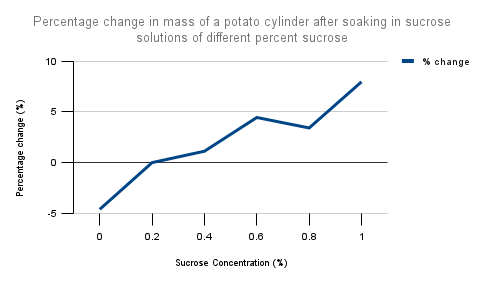
\includegraphics[width=0.7\textwidth]{RPA3-GRAPH.png}
    \caption{Graph showing Percentage chains in mass}
\end{figure}

\subsection{Calculating results}
To calculate the Percentage change in mass, I used the equation\\ $\mbox{Percentage Change in Mass} = \frac{\mbox{Change in mass}}{\mbox{Original mass}}\times 100$

\section{Question}
\begin{enumerate}
    \item \textbf{Why are they dried very carefully?} \\ The potato is dried carefully so it's not damaged.
    \item \textbf{Explain why the potato chips are left in the solution for 20 minutes. After 20 minutes what happens to the net diffusion of water molecules?} \\ They are left in the solution for 20 minutes so there is a chance for the net diffusion of water molecules to have reached dynamic equilibrium.
    \item \textbf{Why are the potato chips dried before they are re-weighed?} \\ The cylinders are dried before re-weighing to remove any surface liquid.
    \item \textbf{Why was change in mass data converted into percentage change in mass in this investigation?} \\ The change in mass data was converted into percentage change in mass so the difference in starting weights of the potatoes doesn't matter.
    \item \textbf{Use your graph to find which molarity of sucrose solution has the same water potential as the potato. Explain how you got your answer.} \\ 0.2\% sucrose solution has the same water potential as the potato because there is no mass change.
    \item \textbf{Explain fully the shape of the graph in terms of water potential (i.e. why some potato chip gain mass, why some lose mass and why some may stay the same.)  In your answer, use the following terms: Osmosis, water potential, water potential gradient, net movement of water molecules.} \\ Some potato cylinders loose mass because they start with a higher water potential than the solution than the solution, so the net movement of water molecules is from the potato to the solution. Other potato cylinders gain mass, this is because the water potential gradient goes from solution to potato, meaning water molecules move from solution to potato by osmosis.
    \item \textbf{What is your estimate of the water potential of potato chips used?} \\ -0.55
    \item \textbf{Explain how you obtained a value for the water potential of the potato used.} \\ Use a water potential calibration curve
    \item \textbf{How could you increase the reliability of this investigation?} \\ Repeat it multiple times 
\end{enumerate}

\end{document}
